\begin{figure}[H]
\centering
\resizebox{0.52\linewidth}{!}{
\begin{tikzpicture}[
 scale=0.50,
  every node/.style={transform shape}, 
  node distance=11mm,
  box/.style      ={rectangle, draw, rounded corners, align=center,
                    minimum width=44mm, minimum height=9mm},
  decision/.style ={diamond, aspect=2.2, draw, align=center, inner sep=1.4pt},
  ->, >=Latex
]

%--- Main process node ------------------------------------------------------
\node[box]      (model)   {\textbf{Define/Revise a model}};

\node[box]      (checking1)  [below=of model] {\textbf{Model checking} \\
(Simulate with $\lambda_0$; fit model; recover $\lambda_0$?)};

\node[decision] (pass1)   [below=10mm of checking1] {\textbf{Plausible?}};

\node[box]      (fit)     [below=of pass1]  {\textbf{Fit to real data}\\
(Compute posterior)};

\node[box]      (gen)     [below=of fit]    {\textbf{Posterior predictive model checking}\\
(Generate fake data from Posterior)\\
(Compare fake vs real)};

\node[decision] (pass2)   [below=of gen] {\textbf{Adequate?}};

\node[box]     (report)  [below=of pass2] {\textbf{Report/Interpret}};

%--- 连线 ------------------------------------------------------------
\draw (model)   -- (checking1)
      (checking1)  -- (pass1)
      (pass1)   -- node[right]{Yes}(fit)
      (fit)     -- (gen)
      (gen) -- (pass2)
      (pass2) -- node[right]{Yes}(report);

%--- Loopback ------------------------------------
\draw[->] (pass1.west) -- ++(-30mm,0) |- (model.west) node[pos=0.23, left]{No};
%\draw[->] (pass1.west) to[out=180,in=180,looseness=1.3] node[left]{No} (model.west);
\draw[->] (pass2.east) -- ++ (30mm,0 )|- (model.east) node[pos=0.23,right]{No};
\end{tikzpicture}}
\caption{General Bayesian workflow}
\end{figure}

\begin{tcolorbox}[
  title  = Algorithm 1: Simulating a Fake Survival Dataset (e.g.Posterior predictive model checking),
   fonttitle  = \small, 
  colback = white,
  colframe=black]
\textbf{Input}\\
\quad$\bullet$ posterior samples $\{\lambda^{(s)}\}$ \hfill (obtained by fitting real data)\\
\quad$\bullet$ sample size $n$ \hfill (same size as the real data set)\\
\quad$\bullet$ start‑time range $[a,0]$ with $a<0$ \\[6pt]
\textbf{Algorithm}\par
\begin{enumerate}
  \item Choose a single $\lambda^\ast$ from posterior samples \hfill (e.g.\ posterior mean)
  \item For $i = 1,\dots,n$
        \begin{enumerate}
          \item[] \hspace*{-10pt}%
          \begin{minipage}[t]{\linewidth}
          \begin{enumerate}
            \item Draw latent duration: $y_i \sim \operatorname{Exp}(\lambda^\ast)$
            \item Draw start time: $T_i \sim \operatorname{Uniform}(a,0)$
            \item Compute leaving time: $t_i = T_i + y_i$
            \item Observed pair $(\text{time}_i,\text{event}_i)$ \[\begin{aligned}
\text{if } \quad t_i &< 0: &&&\text{(event occurred before now)}\\
  &&\quad  \text{event}_i=1, &&\text{(uncensored)}\\ 
  &&\quad \text{time}_i=y_i
   &\quad \\
&\text{else}: &&&\text{(event in the future)}\\
   &&\quad \text{event}_i=0, &&\text{(right censored)}\\ 
   &&\quad \text{time}_i=-T_i &&\text{(time already spent)}
   &\quad 
\end{aligned}\]
          \end{enumerate}
          \end{minipage}
        \end{enumerate}
  \item Combine $(\text{time}_i,\text{event}_i)$ into a fake data set of size $n$.
\end{enumerate}
\label{fake data}
\end{tcolorbox}

\subsubsection{Model Checking via ECDF under Independent Censoring}
In model checking, to compare the overall distributional shapes of the real data and the simulated data, we use the empirical cumulative distribution function (ECDF) rather than histograms. Unlike histograms, ECDFs do not depend on subjective choices of bin widths and break points, thereby avoiding visual biases. Moreover, an ECDF is a monotone right-continuous step function defined on $[0,\infty)$, which stably displays differences between samples over the entire time axis. Importantly, ECDFs can be plugged directly into distance statistics such as the Kolmogorov–Smirnov or Cramér–von Mises metrics, facilitating quantitative assessment of model fit.

In survival data, the observed duration is determined jointly by the latent event time $T\ge 0$ and the censoring time $C\ge 0$. The observed quantity is
$$
Y=\min(T,C),\qquad \delta=\mathbf 1\{T\le C\}.
$$
That is, we observe the event time only when it is uncensored; otherwise, we observe the censoring time. Consequently, we split the data into two subsamples—an “event subsample’’ with $\delta=1$ and a “censored subsample’’ with $\delta=0$—and compute ECDFs for each subsample separately.

Under independent (non-informative) censoring, i.e., $T\perp C$, the two subsamples may be viewed as arising from two conditional distributions
\begin{itemize}
    \item for the event subsample ($\delta=1$), the observed values $Y=T$ follow the conditional distribution $T\mid(T\le C)$;
    \item for the censored subsample ($\delta=0$), the observed values $Y=C$ follow the conditional distribution $C\mid(C<T)$.
\end{itemize}
Let the event-subsample size be $n_1=\sum_i \delta_i$ and the censored-subsample size be $n_0=\sum_i (1-\delta_i)$. The corresponding empirical distribution functions are
\begin{equation}
    \widehat H_{\text{event}}(t)
=\frac{1}{n_1}\sum_{i:\,\delta_i=1}\mathbf 1\{Y_i\le t\},\qquad
\widehat H_{\text{cens}}(t)
=\frac{1}{n_0}\sum_{i:\,\delta_i=0}\mathbf 1\{Y_i\le t\},\qquad t\ge 0.
\end{equation}
By the Glivenko–Cantelli theorem (\cite{tucker1959generalization}), as sample sizes grow, these ECDFs converge uniformly to their respective target distribution functions
\begin{align}
\widehat H_{\text{event}}(t) &\xrightarrow{\text{uniformly in } t} H_{\text{event}}(t) := \Pr(T \le t \mid T \le C) \\
\widehat H_{\text{cens}}(t) &\xrightarrow{\text{uniformly in } t} H_{\text{cens}}(t) := \Pr(C \le t \mid C < T)
\end{align}
In summary, by splitting the data into event and censored subsamples and plotting their empirical distribution functions $\widehat H_{\text{event}}$ and $\widehat H_{\text{cens}}$, we can evaluate model fit within a unified framework along both dimensions.



%%%%%%%%%%%%%%%%%%%%%%%%%%%%%%%%%%%%%%%%%%%%%%%
\subsubsection{Choosing and Interpreting the Survey-Length Parameter $A$}

In the posterior predictive model checking of this study, we generate simulated data from the model and compare it with the observed data. This simulation relies on sampling given known quantities; a key quantity is the \textbf{maximum survey duration $A$ }in Algorithm 1 (\ref{fake data}), which is controlled by the user-specified parameter $a$, with the reparameterization $A = -a$, governing the censoring mechanism in the simulated data. In other words, $A$ sets the observation window in simulation and thereby affects both the censoring rate and the distribution of event times.

This quantity is not a parameter to be estimated by the model; it is an external input required to generate fake data. Although it may appear auxiliary, it is tightly coupled with model checking—different choices of $A$ change the censoring structure of the simulated data and therefore influence the credibility of posterior predictive results.

Does the observed data carry information about $A$? Yes. In any survival dataset, the “shadow” of the survey window is reflected in the censoring proportion and the shape of the observed durations. If the survey is short (small $A$), many subjects are censored before the event occurs, leading to a high right-censoring rate and “compressed” event times. Conversely, with a long survey (large $A$), more events are observed, censoring decreases, and event times spread out.

This can be seen in Figure~\ref{fig:离职数据分开的直方图} (histograms of event and censored durations in the employee turnover data). The number of events and censors is roughly balanced, suggesting that the survey was long enough to capture about half of the departures. Since the maximum observed duration exceeds 170 months, it is reasonable to infer that the underlying survey duration $A$ should be at least greater than 170; this directly informs how the censoring mechanism should be set in simulation.
\begin{figure}[H]
    \centering
    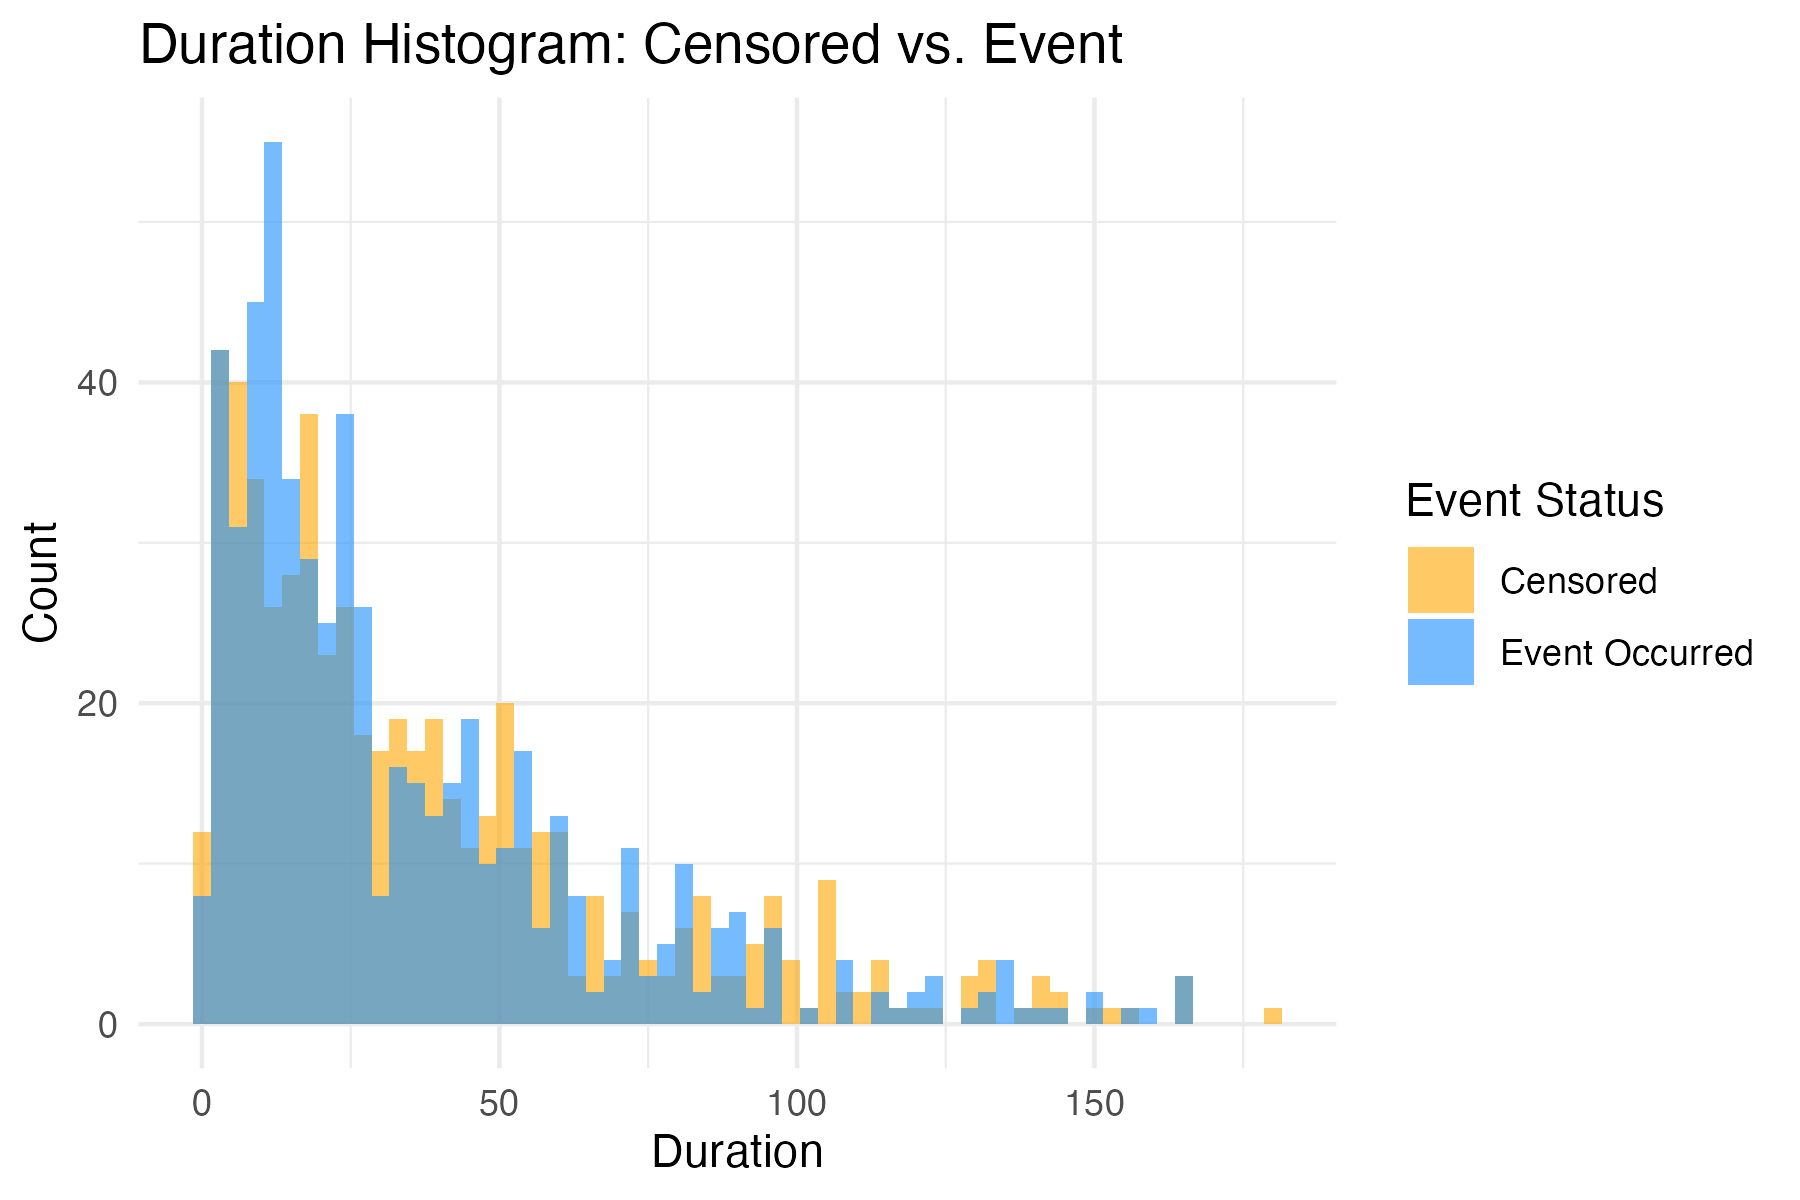
\includegraphics[height=5.5cm, width=0.6\textwidth]{images/separate_hist.png}
    \caption{Histograms of censored and event durations in the employee turnover data}
    \label{fig:离职数据分开的直方图}
\end{figure}
To further support this point, we simulate under two settings, $A = 30$ and $A = 1000$, and plot the empirical cumulative distribution functions (ECDFs) for both the event subsample ($\delta = 1$) and the censored subsample ($\delta = 0$), along with the histograms of simulated durations.
\begin{itemize}
    \item $A = 30$ (Figure~\ref{fig:ppc-A30}). Compared to the real-data histogram (Figure~\ref{fig:离职数据分开的直方图}), the simulated durations in Figure~\ref{fig:fake-hist_a30} are heavily compressed within 0–30 months, indicating that both events and censorings occur unusually early. Correspondingly, the ECDFs for events and censorings (Figure~\ref{fig:ecdf-cens_a30}~\ref{fig:ecdf-event_a30}, red lines) rise too steeply at short durations, deviating noticeably from the observed curves. This mismatch is primarily driven by an unrealistic observation window $A$, rather than a misfit of the event-time distribution (e.g., the parameter $\lambda$) itself.
    \item $A = 1000$ (Figure~\ref{fig:ppc-A1000})
  In contrast, Figure~\ref{fig:fake-hist_a1000} shows a histogram with a much wider and sparser spread of durations, and the ECDF curves (Figure~\ref{fig:ecdf-event_a1000}~\ref{fig:ecdf-cens_a1000}, red lines) align more closely with the observed data. However, when compared to the real-data histogram in Figure~\ref{fig:离职数据分开的直方图}, this setting exceeds any realistic survey length—implying a maximum tenure close to 83 years—which is implausible in practical employment contexts. Thus, although the simulated curves fit better visually, this apparent “match” relies on an unrealistic assumption about $A$, and should not be accepted as a reliable model-checking result.
\end{itemize}
These two examples reinforce a key point: when performing posterior predictive checks, fit quality must be evaluated alongside the realism of the data-generating assumptions in simulation.
\begin{figure}[htbp]
\centering
\begin{subfigure}[t]{0.3\textwidth}
  \centering
  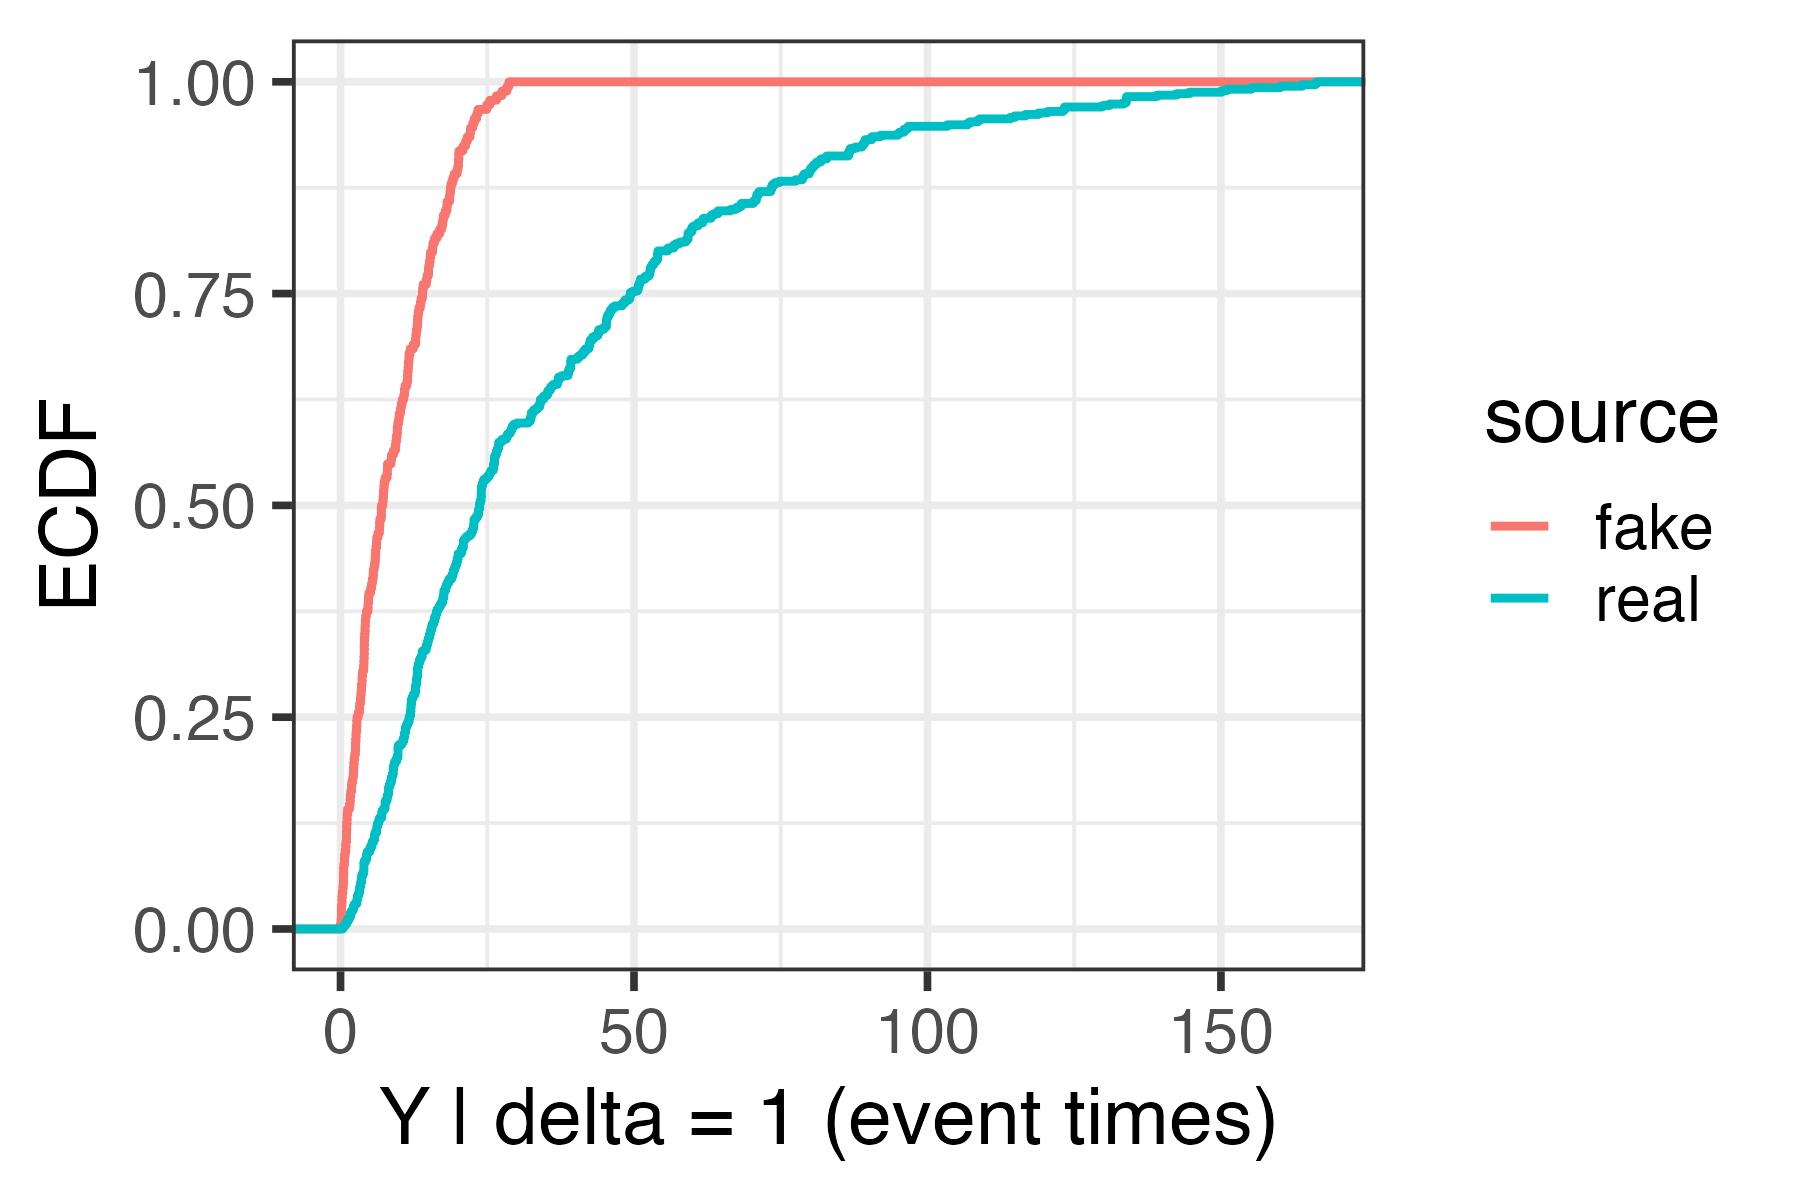
\includegraphics[width=\linewidth]{images/ppc_event_ecdf_A30.png}  % 图1路径
  \caption{ECDF of $Y \mid \delta=1$}
  \label{fig:ecdf-event_a30}
\end{subfigure}\hfill
\begin{subfigure}[t]{0.3\textwidth}
  \centering
  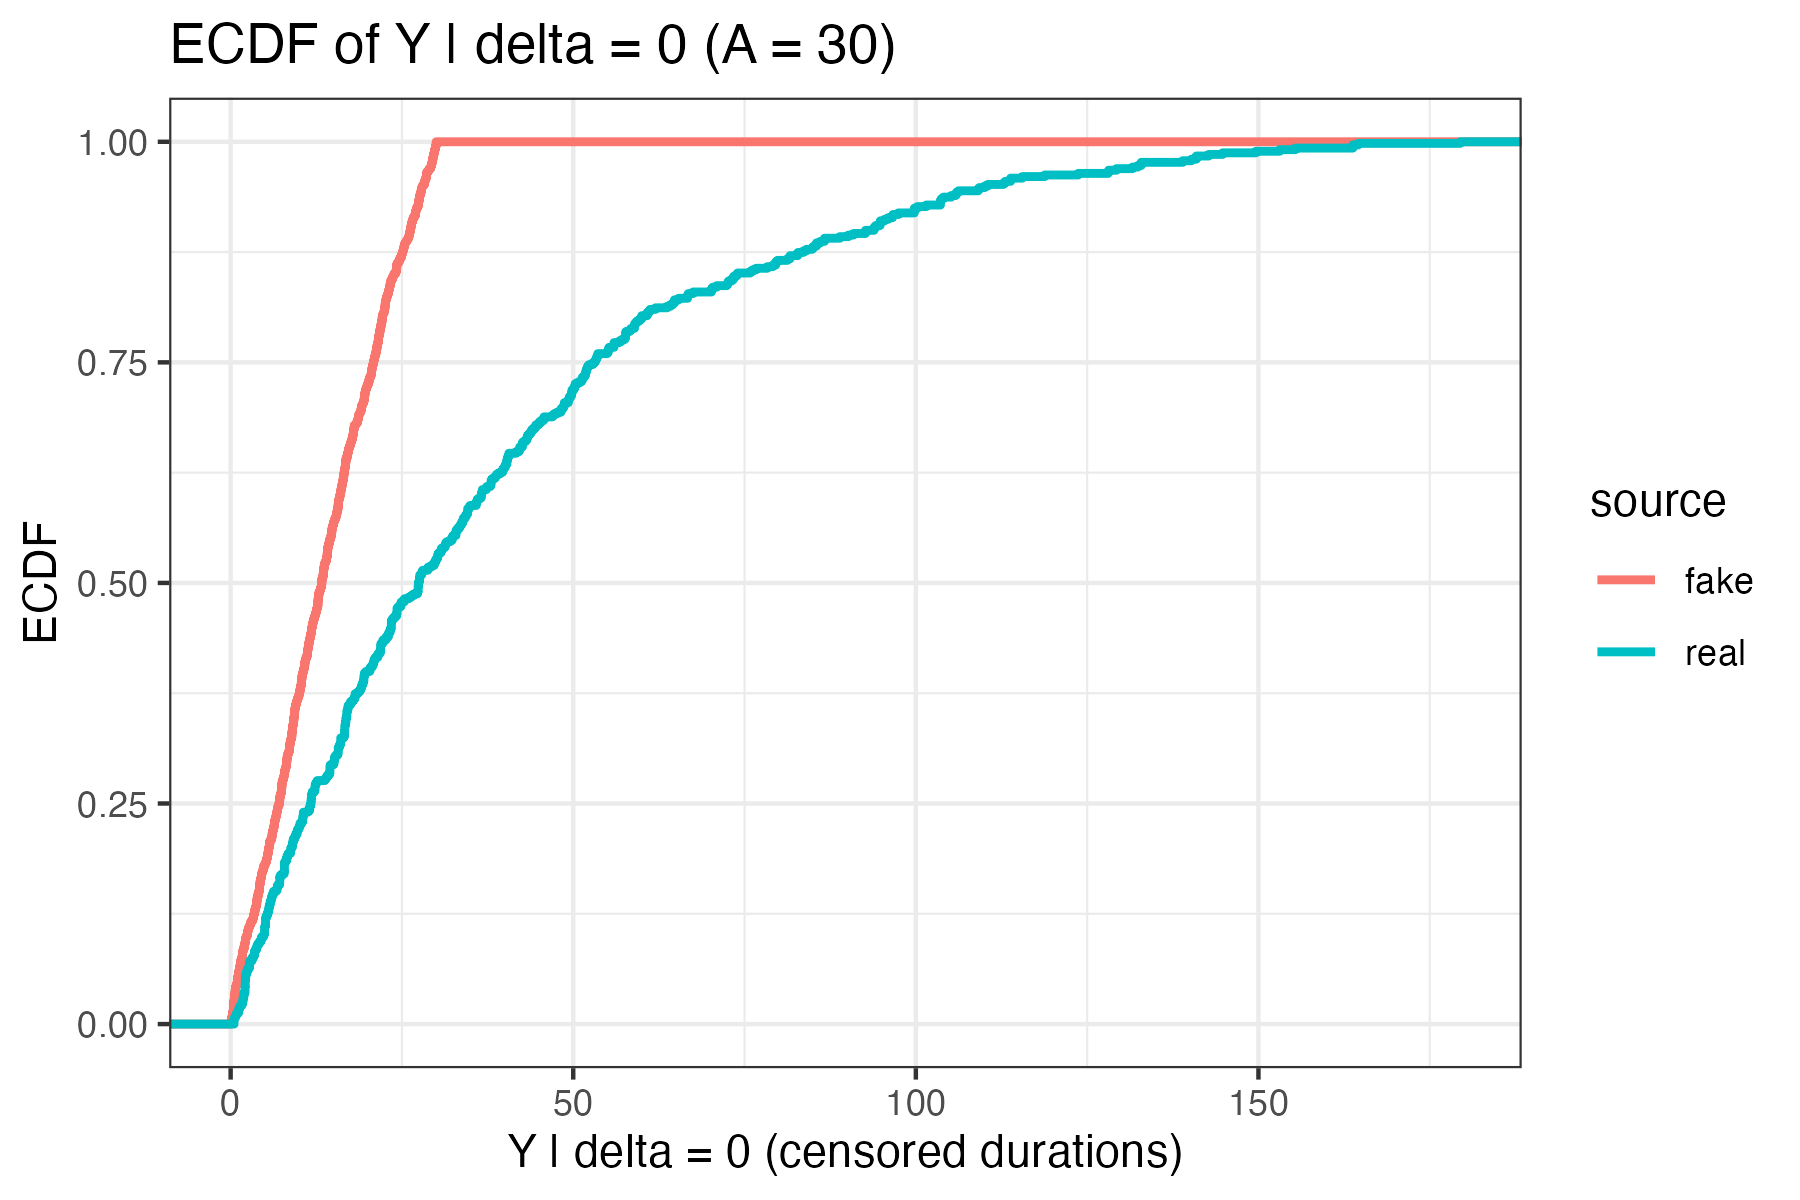
\includegraphics[width=\linewidth]{images/ppc_censored_ecdf_A30.png}   
  \caption{ECDF of $Y \mid \delta=0$}
  \label{fig:ecdf-cens_a30}
\end{subfigure}\hfill
\begin{subfigure}[t]{0.37\textwidth}
  \centering
  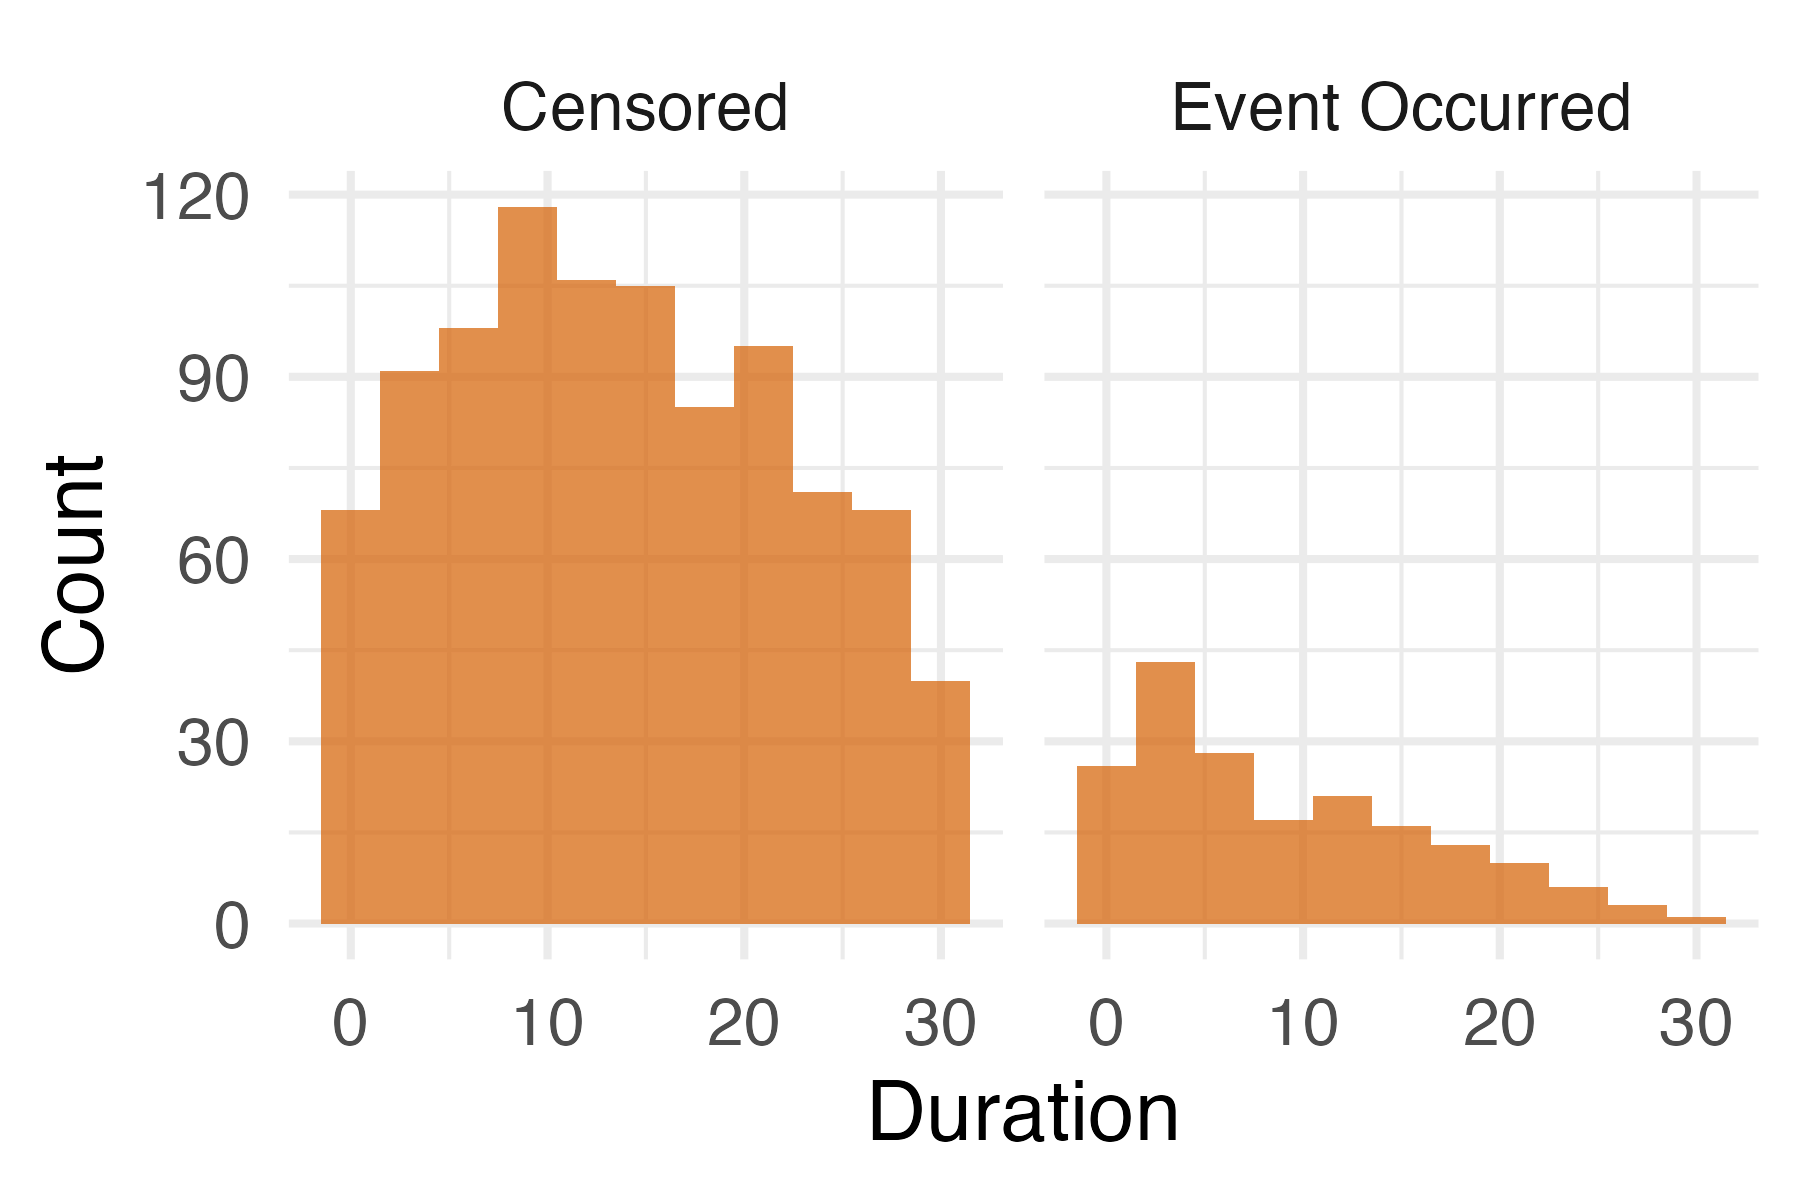
\includegraphics[width=\linewidth]{images/fake_duration_hist_a30.png}   % 图3路径
  \caption{Fake-data histogram}
  \label{fig:fake-hist_a30}
\end{subfigure}
\caption{Posterior predictive checking ($A=30$).}
\label{fig:ppc-A30}
\end{figure}
%%%%%%%%%%%%%%%%%%%%%%
\begin{figure}[htbp]
\centering
\begin{subfigure}[t]{0.3\textwidth}
  \centering
  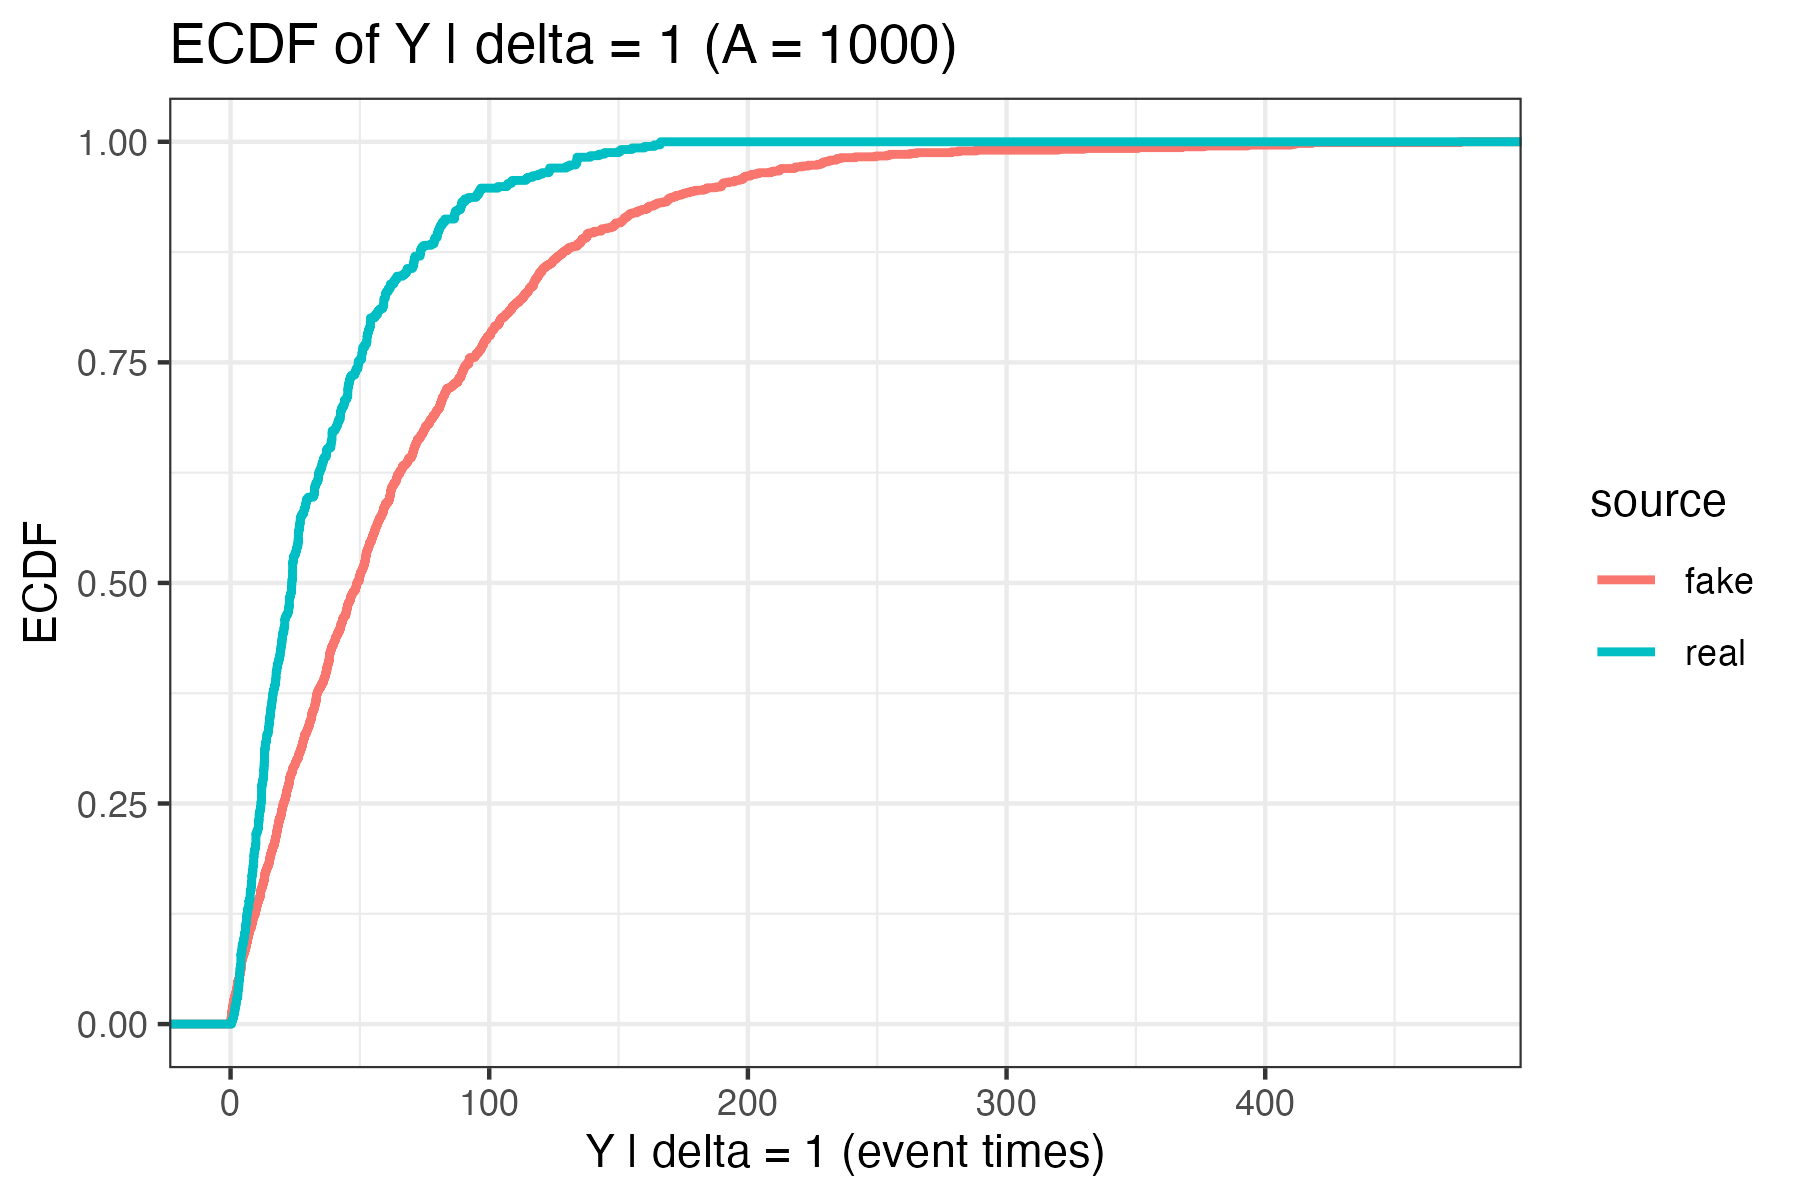
\includegraphics[width=\linewidth]{images/ppc_event_ecdf_A1000.png}  % 图1路径
  \caption{ECDF of $Y \mid \delta=1$}
  \label{fig:ecdf-event_a1000}
\end{subfigure}\hfill
\begin{subfigure}[t]{0.3\textwidth}
  \centering
  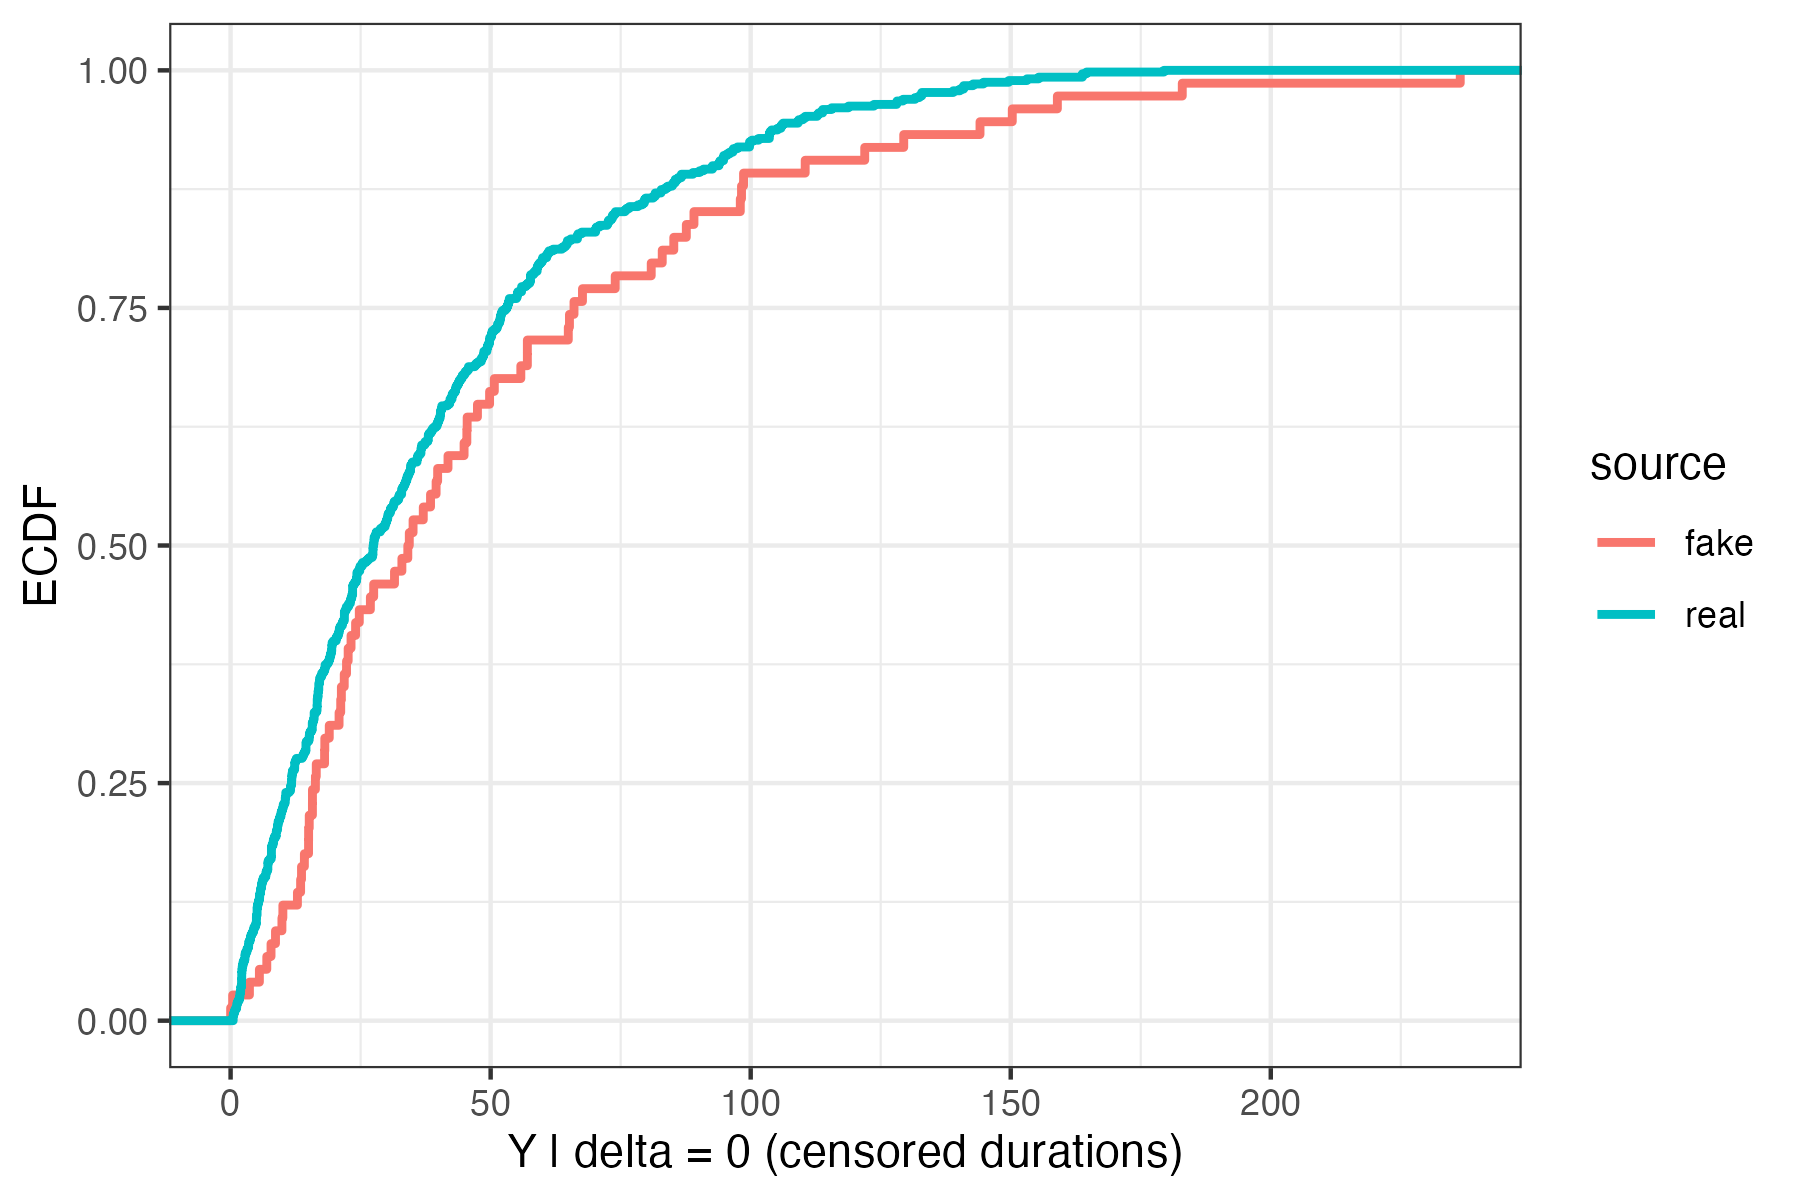
\includegraphics[width=\linewidth]{images/ppc_censored_ecdf_A1000.png} 
  \caption{ECDF of $Y \mid \delta=0$}
  \label{fig:ecdf-cens_a1000}
\end{subfigure}\hfill
\begin{subfigure}[t]{0.37\textwidth}
  \centering
  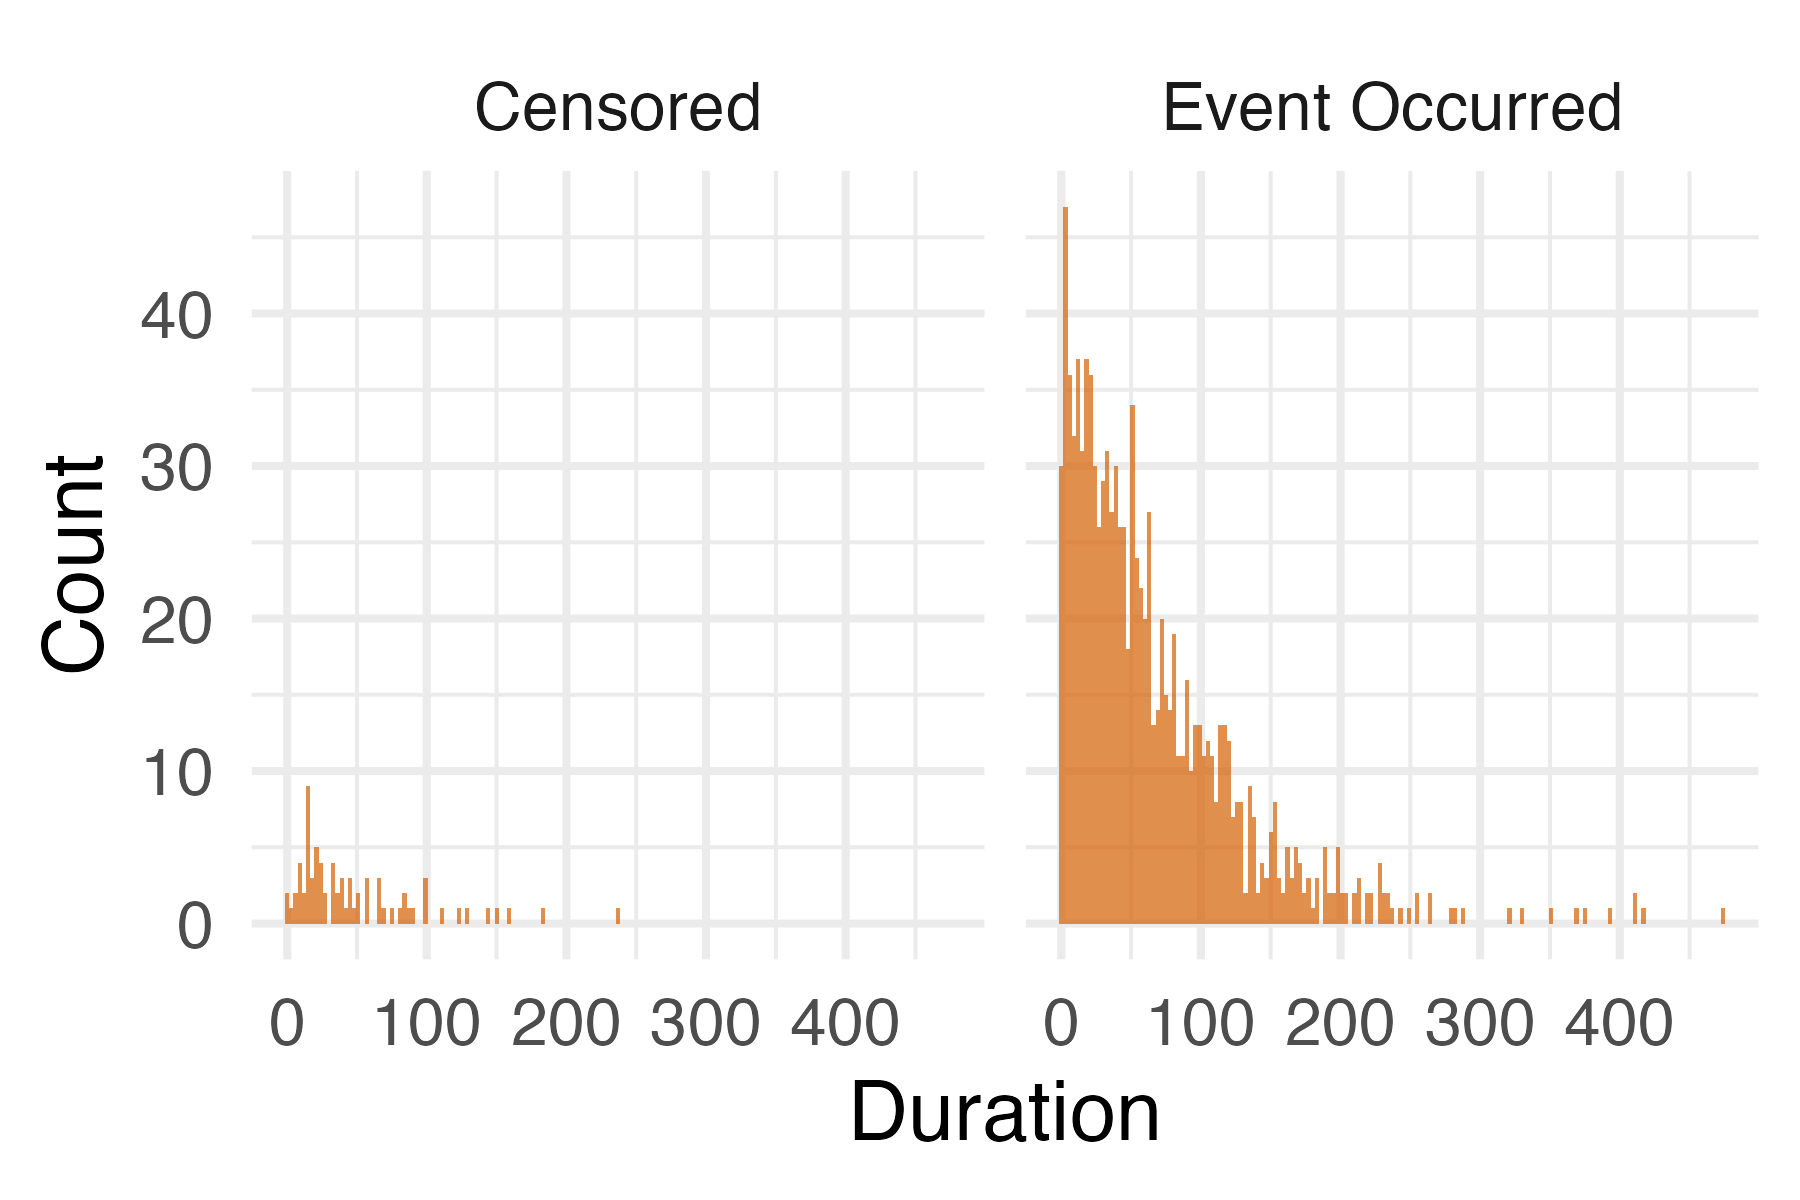
\includegraphics[width=\linewidth]{images/fake_duration_hist_a1000.png}   % 图3路径
  \caption{Fake-data histogram}
  \label{fig:fake-hist_a1000}
\end{subfigure}
\caption{Posterior predictive checking ($A=1000$).}
\label{fig:ppc-A1000}
\end{figure}


%\subsection{Posterior predictive CDF}
%\input{MSc_Statistics_Research_Report_paper/section/Methods_subsection/posterior predictive cdf }




